\begin{figure}
\centering
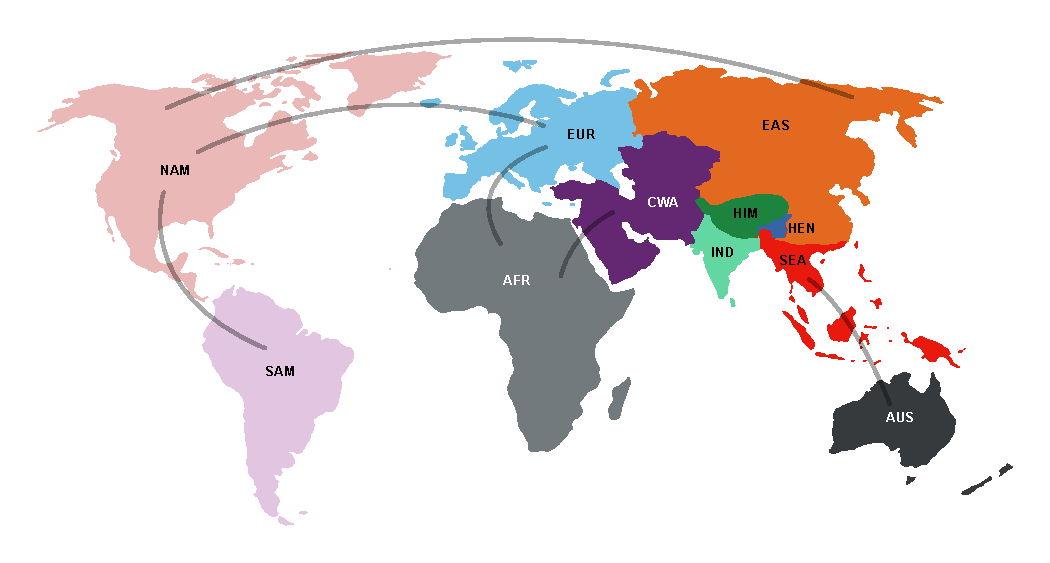
\includegraphics[width=.99\linewidth]{figures/regions.pdf}
\caption{Map of the 11 geographic regions used for ancestral range
  analyses in Lagrange.  HEN = Hengduan Mountains, HIM =
  Himalayas-QTP, EAS = temperate/boreal East Asia, SEA = Southeast
  Asia, CWA = Central/Western Asia, EUR = Europe, IND = India, AFR =
  Africa, NAM = North America, SAM = South America, AUS =
  Australasia. Lines and common borders indicate dispersal routes
  allowed in Lagrange.}
\label{fig:regions}
\end{figure}

%%% Local Variables:
%%% mode: latex
%%% TeX-master: "SI"
%%% End:
